\documentclass[IEEEtran,letterpaper,10pt,titlepage,draftclsnofoot,onecolumn]{article}

\usepackage{nopageno}
\usepackage{alltt}
\usepackage{float}
\usepackage{color}
\usepackage{url}
\usepackage{balance}
\usepackage{enumitem}
\usepackage{pstricks, pst-node}
\usepackage{geometry}
\geometry{textheight=9.5in, textwidth=7in}
\newcommand{\cred}[1]{{\color{red}#1}}
\newcommand{\cblue}[1]{{\color{blue}#1}}
\usepackage{hyperref}
\usepackage{textcomp}
\usepackage{listings}
\usepackage{graphicx}
\graphicspath{ {images/} }

\definecolor{dkgreen}{rgb}{0,0.6,0}
\definecolor{gray}{rgb}{0.5,0.5,0.5}
\definecolor{mauve}{rgb}{0.58,0,0.82}
\lstset{frame=tb,
  language=c,
  aboveskip=3mm,
  belowskip=3mm,
  showstringspaces=false,
  columns=flexible,
  basicstyle={\small\ttfamily},
  numbers=none,
  numberstyle=\tiny\color{gray},
  keywordstyle=\color{blue},
  commentstyle=\color{dkgreen},
  stringstyle=\color{mauve},
  breaklines=true,
  breakatwhitespace=true,
  tabsize=3
}

\def\name{Zach Rogers}

\begin{document}
\begin{titlepage}
  \begin{center}
    \vspace*{1cm}

    \huge
    \textbf{Technology Review - Security for Robotics}
  \vspace{0.5cm}

    \textit{Zach Rogers}\\
  \vspace{0.5cm}
    \vfill
    \large
    \textbf{CS461 Capstone}\\
  \vspace{5mm}

    \textbf{16 Nov 2016}\\

    \vfill
    \end{center}
\end{titlepage}

\begin{abstract}
Our goal as a group is to identify vulnerabilities, both hardware and software related, within our drone system.
A big part of that will have to do with the drone's communication channel, which describes how a user controls a
drone during flight and general operation. In order to attack the communication channel, we must first understand
how the drones communicate with the user, and how the user sends commands to the drone. This will involve lots of
data capturing. So my focus right now is to determine how we will be capturing that data, and how we will use that
data to reverse-engineer the drone's methods of communication for the purpose of developing attack methods.
\end{abstract}

\hrule\vspace{5mm}
\subsection*{Drone Communication Channel}
The two drones that we have use a 2.4Ghz data-link between the drone and the receiver ground-station unit.
That receiver unit then uses a Bluetooth connection to connect to the user's controller, which is a physical controller
or device such as a laptop or tablet.\cite{NazaM2} With this in mind, there are two communication channels that can be
targeted; the connection from the drone to the ground-station unit, and the connection from the ground-station unit
to the controller, this can be seen on Figure ~\ref{fig:datalink_diagram}\cite{NazaM2}.

\begin{figure}[h]
  \makebox[\textwidth]{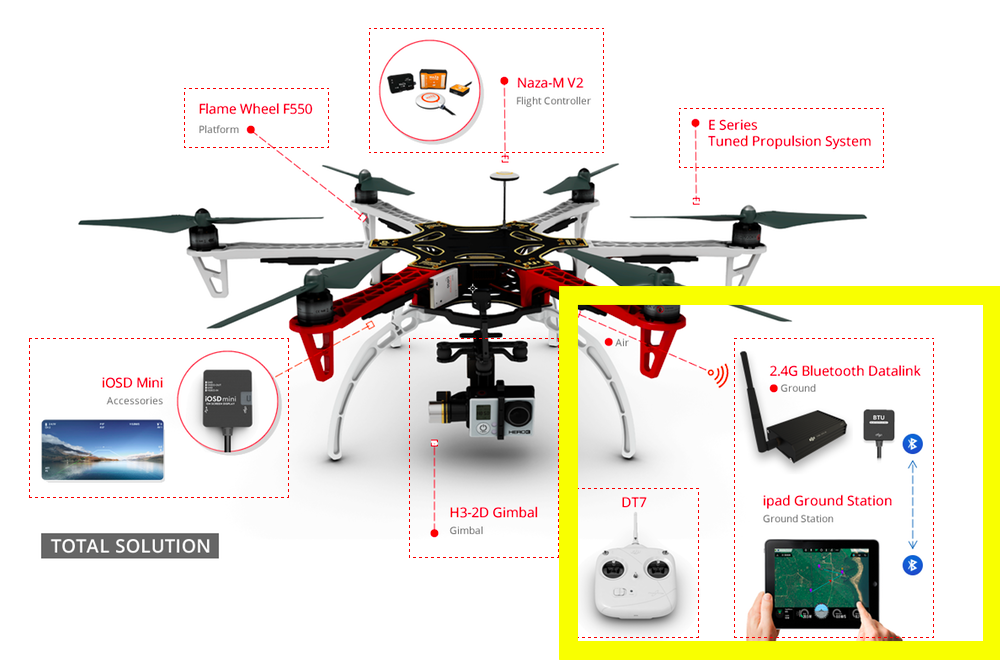
\includegraphics[width=\paperwidth]{datalink_diagram}}
  \caption{Flame Wheel ARF F550 Datalink Diagram}
  \label{fig:datalink_diagram}
\end{figure}

The 2.4Ghz frequency is commonly used by most Wireless Access Points, following the IEEE 802.11a/b/g
standard. Bluetooth is another protocol that operates within the 2.4Ghz RF (radio frequency)
spectrum\cite{HakDaSpectrum}. This means that communication packets for the drone are being sent and received out in the
open, which can be can be intercepted and analyzed with the right tools.

Each drone will be using a BeagleBone Black with a PixHawk Fire v1.6 Cape, making our drones Linux powered, running
Ubuntu Snappy Core, enabling us to use ROS\cite{PixHawk}. The PixHawk is a flight control system, similar to the
Naza-M2, which comes standard on the Flame Wheel ARF F550. It handles the drone's flight system, and includes a cluster
of sensors (GPS, Gyroscope, etc) to keep track of vital information in order to maintain control over the drone while
in flight. The PixHawk also handles telementry communication between the drone and the ground-station. As stated before,
2.4Ghz is the operating frequency between the drone and the ground-station, though the PixHawk also supports a RFD900
900Mhz Telemetry Radio, for longer operating distances\cite{PixHawkDocs}. This opens up an additional communication
channel that could be targeted. In order to intercept and analyze 900Mhz RF communications, we would need additional
tools, seperate from what would be needed to intercept and analyze communications on the 2.4Ghz
frequency\cite{HakDaSpectrum900}.

What should now be clear is that there are a lot of data transmitted in the open air in order to have a successful
drone system. This means that there are a lot of different ways that communications can be intercepted and even
altered, in an attempt to gain control over a drone's flight plan. Knowing which communication channels to target
is only a small part of getting to the ultimate goal of intercepting drone data; consider that the R&D phase. The next
step is to explore how exactly to capture that data.

\subsection*{Methods of Data Capture}


\subsection*{Leveraging Captured Data to Develop Attack Methods}


\newpage
\bibliographystyle{IEEEtran}
\bibliography{tech_review}

\end{document}
